\documentclass{article}

\usepackage[utf8]{inputenc}

\title{Rapid shortening at the eastern margin of the Tibetan plateau prior to the 2008 Mw=7.9 Wenchuan earthquake}
\author{T. Ben Thompson, Brendan J. Meade}
\date{September 2014}
\usepackage{graphicx}
\usepackage[margin=1.0in]{geometry}

\begin{document}

\maketitle

\section{Abstract}
The Longmen Shan is the steepest topographic front of the India-Asia collision and was the site of the Mw=7.9 Wenchuan earthquake. Shortening estimates across the Longmen Shan provide strain accumulation rates and clarify the eastward extrusion of the Tibetan plateau. Here, to explain the interseismic GPS velocities across the greater Longmen Shan region, we develop a boundary element model including earthquake cycle effects, topography, the westward dipping Beichuan fault, and a ~20 km deep, shallowly dipping, detachment. The detachment is inferred from observations of slip during and after the Wenchuan earthquake and from structural considerations. Previous analyses which neglected the detachment and earthquake cycle effects have found shortening rates near zero. In contrast, we find that interseismic GPS data are consistent with a shortening rate of 6$\pm$2 mm/yr. These results suggest that the Longmen Shan is an active fold-and-thrust belt with Wenchuan style earthquake recurrence intervals of $<$600 years.

\section{Introduction}
The Longmen Shan range is located on the eastern margin of the Tibetan and rises 4000m over 30km (CHECK THESE NUMBERS ON GOOGLE EARTH).
The 2008 $\mathrm{M_w}$ 7.9 Wenchuan earthquake ruptured 250km along strike on the Beichuan and Pengguan faults, resulting in approximately XXXXX fatalities (CITE STONE)
Prior geodetic estimates suggest almost zero horizontal shortening (Chen 2000, Shen 2005, Meade 2007, Loveless and Meade 2011), in contrast with the dominant thrust slip-sense during the Wenchuan rupture. 
Other authors reconcile the lack of shortening with the steep topography by appealing a lower crustal inflation tectonic model for the eastern Tibetan Plateau (CITE clark, royden, burchfiel, kirby, etc).
However, the magnitude and location of the Wenchuan earthquake suggest a more typical fold-and-thrust belt. 
Using seismic reflection data, Hubbard and Shaw 2009 find a well-developed fold-and-thrust fault system geometry with long-term shortenings up to 100\%. 
A growing body of literature supports this interpretation, 
Fielding and McKenzie 2012 interpret satellite gravity-field data to infer that mass of the Longmen Shan is supported by a flexed Sichuan Basin. 
This fold-and-thrust structure may extend deep into the plateau as evidenced by seismic tomography and coseismic slip inversions (CITE ZHANG, QI, FIELDING). 
CITE THE PAPERS EXAMINING THE LONGRIBA FAULT THAT PROPOSE A DETACHMENT

However, it remains to be explained how slow present-day geodetic shortening estimates can be reconciled with the Wenchuan earthquake and the large structurally-observed shortening.
Prior estimates can be categorized into those that neglect earthquake cycle effects, analyzing the fault slip-deficit without no explicit model of the geometry or tectonics, (CHEN, SHEN) and those that use block models, which normally assume a simplified fault geometry (CITE MEADE 2007, BURCHFIEL 2008, LOVELESS AND MEADE 2011).
Loveless and Meade report the highest shortening rate of 3.2 mm/yr.
Here, we present a model that includes earthquake cycle effects to explain the regional geodetic velocities as the result of a complex interseismically locked fault geometry, including a 20km deep detachment and the range-front thrust Beichuan fault.
This geometry is consistent with structural interpretations and with the geometry of Qi et al 2012 and Fielding et al 2013. 
Using this range-front thrust plus detachment geometry, we infer an average horizontal shortening between the TIbetan Plateau using interseismic GPS data collected prior to the Wenchuan earthquake.
Next, we show how this geometry can drives the steep velocity gradients far to the northwest of the range front, thus explaining the absence of a range-front interseismic velocity gradient.
Finally, we discuss the effects of Longmen Shan fault geometry on regional seismic hazard and tectonics.

Maybe insert this information? --- Using InSAR measurements and post-Wenchuan GPS observations, Qi et al. 2011 found evidence of 2-6m of slip on a 20km deep detachment that extends 60km northwest underneath the Tibetan Plateau. 

\section{Geodetic analysis of Longmen Shan shortening}

\begin{figure}[h!]
    \centering
    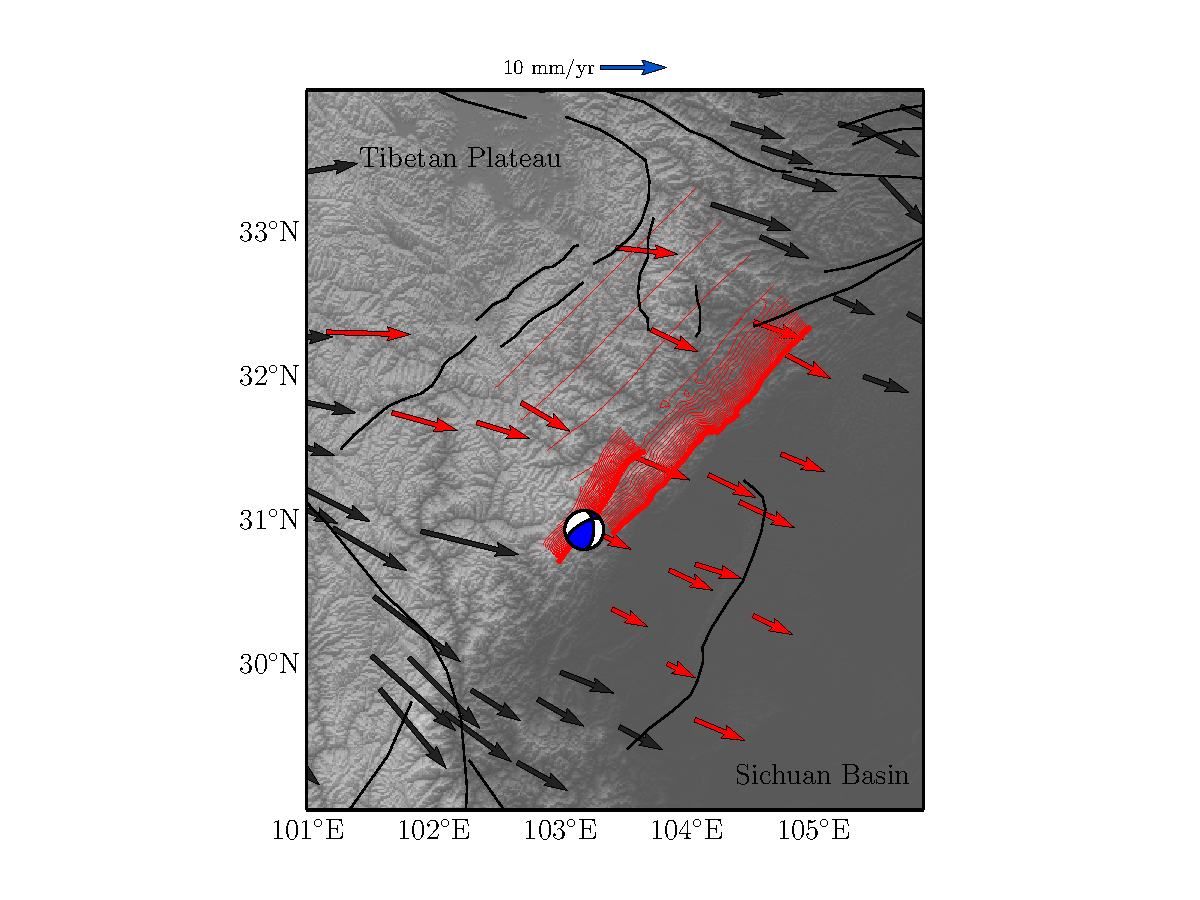
\includegraphics[width=7in]{figs/lms_map_with_faults.pdf}
    \caption{A map of the Longmen Shan region with the basemap showing shaded relief. The focal mechanism plot is located at the epicenter of the Wenchuan earthquake, while the thicker red line shows the surface trace of rupture. The thin red lines show 1km depth contours of our model geometry. GPS velocity vectors are colored black if they are not included in our parameter estimation and red if they are included. The blue line shows the two-dimensional cross-section we study. Thin black lines indicate other significant faults in the region.}
    \label{fig:regional_map}
\end{figure}

Our fault geometry is derived from a Community Fault Model for the Longmen Shan and Sichuan Basin region being actively developed (Plesch and Shaw, personal communication).
This geometry is derived from structural interpretation of both seismic reflection surverys and surface geology (Hubbard \& Shaw).
We make no modifications to the geometry except to take a fault-perpindicular cross-section.
The cross-section and geometry with depth contours are shown in Figure \ref{fig:regional_map}.

Because our model includes a deep detachment, we must include interseismic GPS data deep into the interior of the Tibetan Plateau.
We study GPS observations collected prior to the Wenchuan earthquake by (CITES Apel, Banerjee, Calais, Gan, Vigny), assembled into a single reference frame by Loveless and Meade 2011.
These velocities are shown in Figure \ref{fig:regional_map} along with the site of the Wenchuan earthquake and other regional faults.
We include in our estimation velocities that are within the potential far-field influence of a deep detachment under the easternmost Tibetan Plateau and the Longmen Shan.
We exclude velocities that are near major faults like the Xianshuihe fault or the Kunlun fault. 
Later, we demonstrate that our results are reasonably robust to the specific data set that is studied.
Addition of more recent observations could bias our results due to possible postseismic transient deformation.



To analyze these data, we use a new quasistatic elastic boundary element code.
An important feature of our code is the inclusion of accurate surface topography in steep mountain ranges or Earth curvature in large-scale problems.
In addition, we can accurately reproduce half-space solutions to very high precision. 
The steep topography of the Longmen Shan range front is included via the SRTM-30 dataset (CITE SANDWELL).

As demonstrated by the leveling-off of the model predicted velocities, velocities deeper into the plateau are likely controlled by other fault systems.

The debate over shortening in the Longmen Shan has centered around the clear lack of velocity gradient at the range front. 
Chen et al. 2000 < 3mm/yr of shortening in the Longmen Shan.
However, all their stations are within 50km of the range front. CHECK THIS
Reference the plot of GPS velocities in the figure which shows the best fitting solution.
General theme of previous interpretations: either ignored earthquake cycle effects or only looked at the near-field GPS.
Which, if there is a deep detachment, are useless because they would indicate almost no shortening.
Observations may also have been diminished because they were late in the earthquake cycle – just before Wenchuan.
Interseismic locking leads to a smooth profile of geodetic velocities across a locked fault.
Interpreting this profile is highly dependent on fault geometry.
In the Longmen Shan, a deep detachment leads to a surface velocity gradient that is localized very far to the west of the range front.
However, ignoring the detachment would indicate minimal shortening across the range front (see figures).

Our fault geometry is based on a community fault model of the Longmen Shan fault system (in development, shaw, plesch) that is based on seismic reflection imagery.
Although not directly observed, based on structural considerations, they include the deep detachment.
The location of this detachment is approximately the same as the Qi et al. 2011 detachment. We use the SRTM30\_Plus global DEM(becker, sandwell et al.)  to provide a representative, smoothed, topographic profile across the range. 
I need to talk to John Shaw to get reasonable elastic moduli for the region.
For topography, GPS, and fault geometry, we project the data onto the vertical plane of the cross section line (this should just go in a figure).
We fit the GPS velocities with a constant shortening rate on the whole Beichuan + detachment. The best fit is ~8 mm/yr (+-!!). 
I need to actually do some fitting to get uncertainties and best fit!

\section{Implications for tectonics and earthquake hazard}
A detachment underneath the Longmen Shan and Tibetan Plateau indicates that the Tibetan Plateau is thrust over the Sichuan Basin. I should read some of the previous literature on this question. Is there any evidence for Sichuan-like crust beneath easternmost Tibet? 
Hence, our detachment-based interpretation of the geodetic velocities supports a block-like interpretation for the tectonics of the eastern Tibetan Plateau. Lower crustal flow may also be able to explain the steep velocity gradient localized to the west of the range front. However, observations of postseismic afterslip on the detachment surface corroborate our  

Longriba fault zone?

I need to calculate recurrence intervals and look up previous estimates for comparison. 
Assuming 5m of slip in the Wenchuan earthquake, a 45 degree dipping fault, and 8mm of shortening: 8*sqrt(2) mm/yr slip deficit -> 5000/8*sqrt(2) = 441 years.
Assuming that all 8 mm/yr of slip-deficit is concentrated on a single 45 degree dipping fault with the same surface area as the Wenchuan earthquake rupture, we calculate a recurrence interval of 450 years.
However, this recurrence interval ignores the presence of other Longmen Shan faults and should be considered as an upper bound. The Beichuan and Pengguan faults are only two members of an imbricated thrust sequence. Interpretations of seismic reflection data (hubbard et al) find multiple other thrusts including a detachment called the Range Front Thrust that extends 50km into the Sichuan Basin. This detachment lies directly under Chengdu, a city of 14 million. The slip-deficit distribution amongst these faults is unknown. Accounting for the subhorizontal Range Front Thrust, which has a large surface area, might seriously reduce our recurrence interval.

150kms west of the Beichuan, there are 3 GPS stations with similar profile location. But, the velocities are significantly different. This indicates some lateral heterogeneity in the orogeny.

The strain accumulating on the detachment may release coseismically or may be released in any number of slower ways. 
An analysis without the detachment would observe almost no horizontal velocity gradient across the Longmen Shan range front. This emphasizes that geometrically accurate fault models can dramatically alter the interpretation of geodetic data. 
Importance of geometry in seismic hazard. Even including earthquake cycle effects, we would estimate almost zero shortening without the presence of the detachment. Raise the impact of detachments on t

\subsection{A hazard lower bound}
There are reasons to believe that the seismic hazard estimate presented here is a low estimate.
First, coseismic and long term slip estimates include (CITE VARIOUS COSEISMIC + DENSMORE) a significant component of strike-slip motion. But, we only model horizontal shortening. 
Second, our two-dimensional model assumes plane strain conditions. 
The approximation will result in under-estimates of the shortening required to produce far-field velocities.
This is because the assumption is equivalent to assuming the fault geometry extends infinitely far along strike, resulting in a fault surface much larger than in reality. 
Third, the modeled range-front thrust is the steeply dipping Beichuan fault. The foreland Range Front thrust aor the shallow detachment beneath Chengdu (CITE HUBBARDSHAW) dip more shallowly, producing a greater total moment deficit.
These first three deficiencies could be remedied through a more geometrically realistic three-dimensional model of the region. However, the data density may not justify such a complex model. 
(MAYBE REMOVE) Also, kinematically consistent three-dimensional modelling of interseismic deformation is an outstanding issue. 
Finally, the shortening rate estimate may be low due to being estimated late in the earthquake cycle (GOOD CITATION FOR THE GENERAL CONCEPT?). 

On the other hand, there are reasons to believe that the strain energy budget in the Longmen Shan region is not entirely released in major earthquakes. Critical-taper wedge theory results in very low friction coefficients for the shallowly dipping detachment in the foreland and the deep detachment (Hubbard,Shaw, Klinger + deep detachment here). Hence, these fault segments are more likely to release significant energy aseismically. Analogously, it has been suggested that the Himalayan range front consumes most of its energy budget aseismically (CITE!!!).

It is also important that the recurrence interval calculation assumed that the entire range-front was ruptured by the Wenchuan earthquake.
However, the southern portion of the Longmen Shan did not rupture during the earthquake. 

\section{Conclusions}
Previous interseismic shortening estimates suggested almost no shortening. This is at odds with the Mw 7.9 Wenchuan earthquake. We clarify this conflict by including earthquake cycle effects and a 20km deep detachment. Our revised interseismic shortening rate is ().
This interpretation of the interseismic GPS velocities unifies the three phases of the Longmen Shan earthquake cycle. The Mw 7.9 Wenchuan rupture and deep postseismic afterslip suggest an active fold-and-thrust belt in the Longmen Shan orogen. Unlike previous interseismic coupling estimates (cite), our model is aligned with this view of the Longmen Shan. 
Our model suggest that Wenchuan-like events have much shorter recurrence intervals. Yikes!

\end{document}
